\section{Ergebnisse}
Im folgenden Kapitel soll Testresultate der einzelnen Netzwerke präsentiert
werden. Als Leistungsmaß wird die Genauigkeit des jeweiligen Modells präsentiert.
Hierfür wird neben eines Genauigkeit-\#Epochen-Plots eine \emph{Confusionmatrix}
verwendet. Zusätzlich soll anhand der \emph{Loss}-Kurven vom Test- und Validierungsdatensatz
Overtraning festgemacht werden.

\subsection{Traningsweise}
Wie bereits im letzten Kaptiel erwähnt werden die
Bilder batchweise geladen und verarbeitet. Hierbei erfolgt auch eine Normierung
der Pixelwerte. Vor dem Beginn eines Tranings werden \emph{Batch-Größe} und
\emph{Learningrate} festgelegt. Letztere wird jedoch, während des Tranings dynamisch
durch die in \textsc{keras} implementierte Funtkion \textsc{ReduceLROnPlateau}
angepasst \cite{keras_ReduceLROnPlateau}. Die Anzahl der Traningsepochen
wird nicht festgelegt, da hier eine \emph{EarlyStopper} eingestetzt wird \cite{keras_EarlyStopping}.
Zusätzlich muss angegeben werden ob $5$ oder $120$ Hunderassen
klassifiziert werden sollen. Alle Traningseinheiten
auf einer Nvidia Grafikarte statt.

\subsection{NN für 5 Hunderassen}
Die NN werden auch auf einem kleineren Datensatz mit lediglich $5$ Hunderassen
getestet, um Verarbeitungszeiten zu reduzieren. Dies ist insbesondere bei
der Hyperparamteroptimierung von \textsc{MiniDogNN} wichtig.
\subsubsection{MiniDogNN -- Hyperparamteroptimerung}
Bei der Hyperparamteroptimerung (HPO) wurden die Einstellung für die $l2$-Regularisierung $l2\ua{value}$,
die Batchgröße $bs$ und die Farbinformation $color$ der Bilder variiert. Der vollständige
Parameterraum lautet, wie folgt:
\begin{equation}
  \label{eq:Parameterraum_MiniDogNN}
  bs\in\left\{2, 5, 10, 15, 17, 25\right\}, \quad l2\ua{value}\in\left\{0.01, 0.001, 0.005, 0.0001\right\}, \quad color\in\left\{rgb, grey\right\}
\end{equation}
Die maximale Größe der Batchgröße wurde durch den Grafikspeicher limitiert.
Als anfängliche Lernrate wird $lr=0.001$ gewählt.
Das Ergebnis der HPO ist in Abbildung \ref{fig:Hyperraum_MiniDogNN} dargestellt,
deutlich ist der positive Einfluss der Farbinformation $color=rgb=\map{True}=1.0$
zu erkennen.
\begin{figure}
\centering
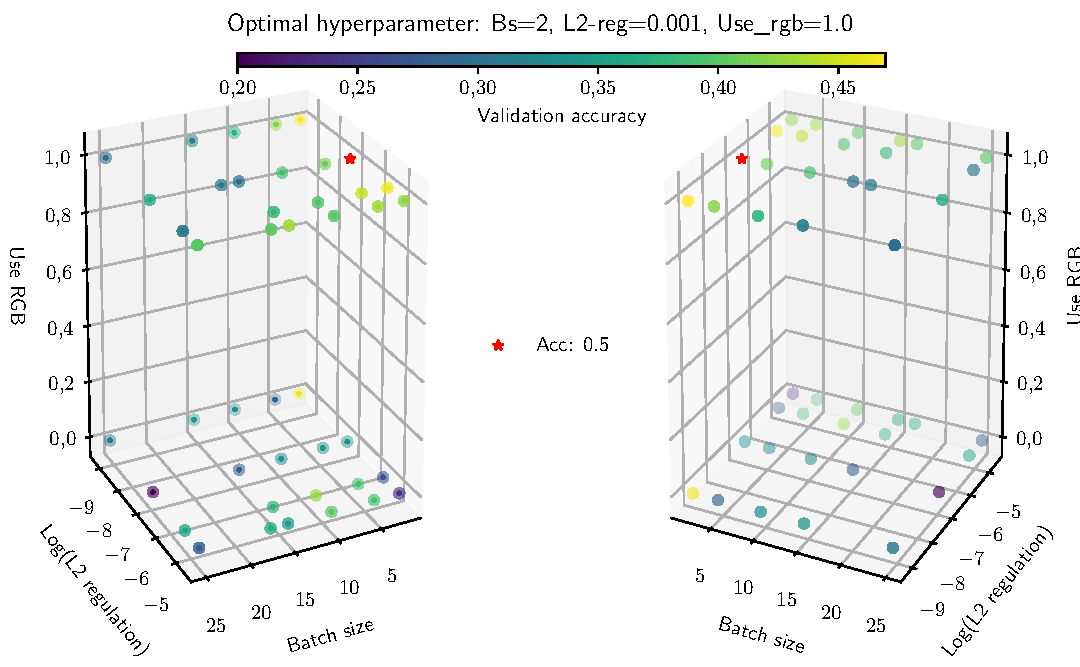
\includegraphics[width=\the\textwidth]{../../final_data/MiniNN_n5/hyper_raum.pdf}
\caption{Ergebniss der HPO, die $z$-Achse \emph{Use RGB} gibt an, ob Farbinformation
          verwendet wurden. Aus den möglichen Paramtern ist die bestmögliche Kombination
         lautet: $bs=2, \, l2\ua{value}=0.001, \, color=rgb$.}
\label{fig:Hyperraum_MiniDogNN}
\end{figure}
Von den $48$ möglichen Kombinationen wurden $43$ erfolgreich beendet, die Restlichen
wurden auf Grund von Grafikspeicherproblem von \textsc{keras} abgebrochen. Eine
Genauigkeitsverteilung ist in Abbildung \ref{fig:Genauigkeitverteilung_MiniDogNN} zu erkennen und verdeutlicht,
dass HPO einer signififikante Genauigkeitsteigerung verursachen kann.
\begin{figure}
\centering
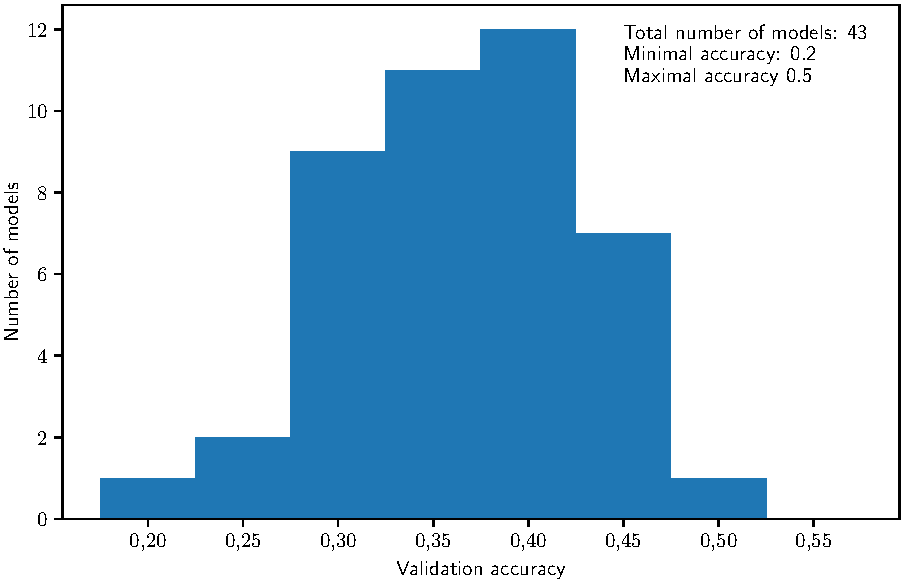
\includegraphics[width=\the\textwidth]{../../final_data/MiniNN_n5/acc_hist.pdf}
\caption{Genauigkeitverteilung der erfolgreich tranierten Modelle der HPO.}
\label{fig:Genauigkeitverteilung_MiniDogNN}
\end{figure}
Es wird der Einfachheit angenommen, dass das Ergebnis der HPO, trotz anderem
FCN, sowohl für das fünf als auch für das 120 Rassen MiniDogNN gilt.

\subsubsection{MiniDogNN}
Als Traningsparameter werden nach der HPO gewählt.
Die Traningsdokumentation findet sich in Abbildung \ref{fig:MiniDogNN_Loss_Acc}.
In dem Plot ist zu erkennen, dass die Architektur geringfügig Übertraniert
wurde.
\begin{figure}
\centering
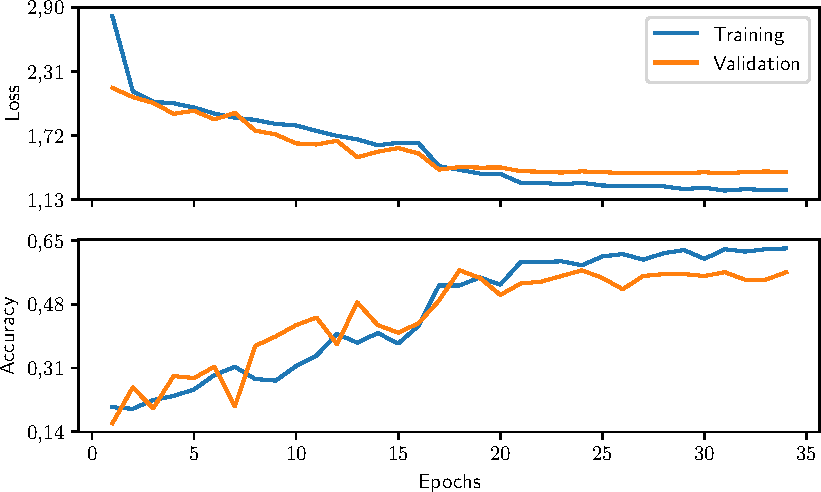
\includegraphics[width=\the\textwidth, scale=0.6]{../../final_data/MiniNN_n5/history.pdf}
\caption{Traningsfortschritt des \textsc{MiniDogNN}.}
\label{fig:MiniDogNN_Loss_Acc}
\end{figure}
Bei Betrachtung der Confusionmatrix in Abbildung \ref{fig:MiniDogNN_Konfusionmatrix} fällt auf, \textbf{dass}
\begin{figure}
\centering
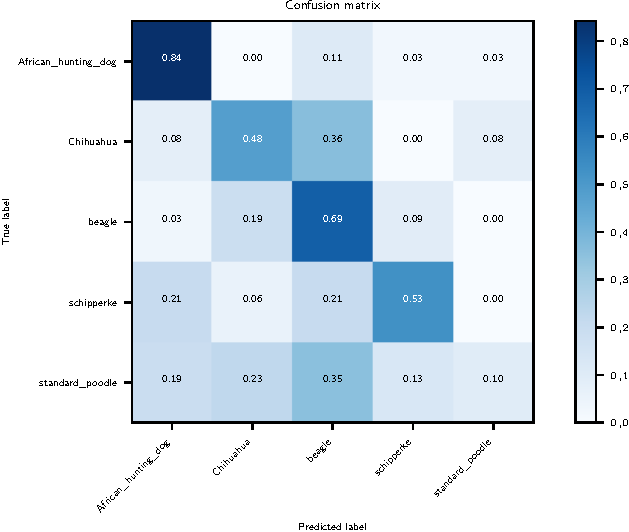
\includegraphics[width=\the\textwidth, scale=0.6]{../../final_data/MiniNN_n5/confusion_matrix_mini.pdf}
\caption{Konfusionmatrix des \textsc{MiniDogNN}.}
\label{fig:MiniDogNN_Konfusionmatrix}
\end{figure}
\subsubsection{PreDogNN}
Die \textsc{PreDogNN}-Architektur wurde mit einer Batachgröße von $16$, einer
$l2$-Regularisierungsstärke von $l2\ua{value}=0.01$, einer Lernrate von
$lr=0.001$, einer Dropourate von $dr=0.2$ und als Farbmodus $color=rgb$ gewählt.
Auf Grund der Verwendung von Dropout muss der Loss und die Genauigkeit nach jeder
Epoche traniert werden, da sich durch Dropout die Struktur des Netzes epochenweise
ändert. Die resultierenden Loss- und Genauigkeitverläufe befinden sich in Abbildung
\ref{fig:PreDogNN_Loss_Acc} und die Konfusionmatrix in Abbildung \ref{fig:PreDogNN_Konfusionmatrix}
\begin{figure}
\centering
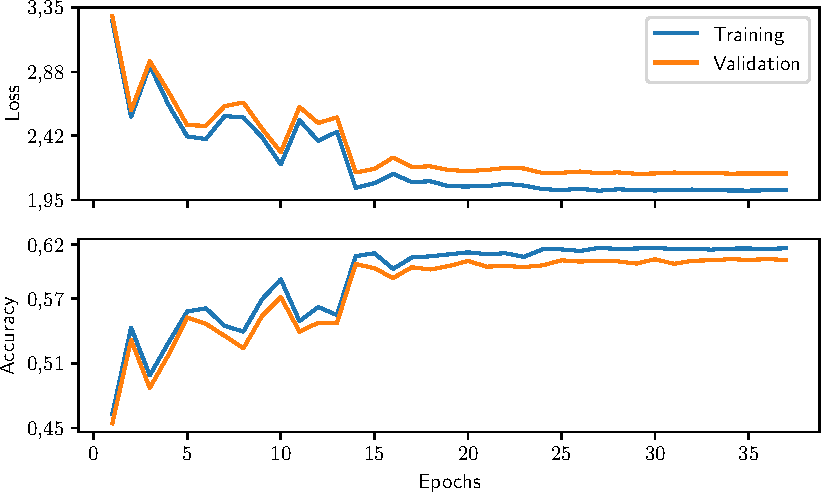
\includegraphics[width=\the\textwidth, scale=0.6]{../../final_data/PreDogNN/16-07-2019_18:39:02/build/history_epoch.pdf}
\caption{Traningsfortschritt des \textsc{PreDogNN}.}
\label{fig:PreDogNN_Loss_Acc}
\end{figure}
\begin{figure}
\centering
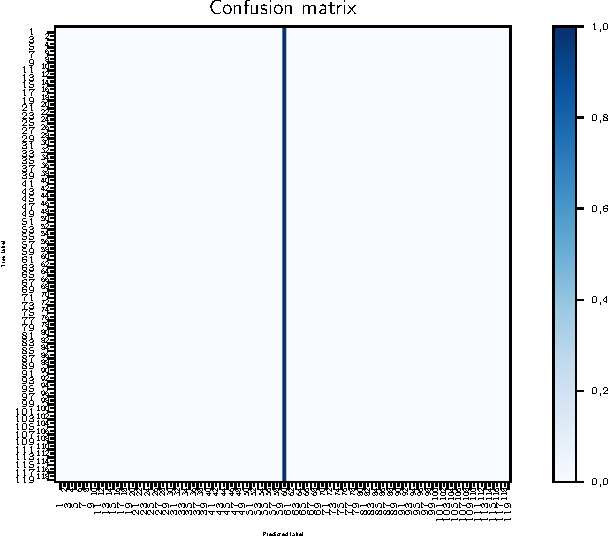
\includegraphics[width=\the\textwidth, scale=0.6]{../../final_data/PreDogNN/16-07-2019_18:39:02/build/confusion_matrix.pdf}
\caption{Konfusionmatrix des \textsc{PreDogNN}.}
\label{fig:PreDogNN_Konfusionmatrix}
\end{figure}
\subsection{NN für 120 Hunderassen}

\subsubsection{MiniDogNN}

\subsubsection{PreBigDogNN}
